% !Mode:: "TeX:UTF-8" 

\BiChapter{绪论}{Figures,Tables and Equations}



%=========================================================================================
\BiSection{研究背景及意义}{Figures}
\label{sec:1.1}

随着互联网技术的发展,如今网络用户由被动变主动成为了网络信息的提供者,在社交网络、电商平台上产生了大量的包含用户观点、态度和情感的主观信息,这些主观性信息主要以文本的形式呈现。运用这些海量的文本信息进行分析,提取出有价值的、包含情感信息的文本,并准确挖掘出其中的情感倾向和原因,有着巨大的应用价值和研究意义  \upcite{lee-etal-2010-text, zhcn_value1, li2017deep}。

情感分析是自然语言处理领域的重要研究方向,情感是人类固有的一部分,自然语言可以反映一个人的情感状态,因此情感识别在自然语言处理领域得到了广泛的应用,例如舆情分析、推荐系统、医疗保健等方面\upcite{zhcn_value2}。情感识别还在计算人类认知过程的建模中扮演着重要角色,其中识别情感原因则是情感分析中的一个重要问题\upcite{wu2006emotion, zhcn_cause}。它可以用来帮助企业或组织了解消费者或用户对其产品或服务的态度和情感。基于深度学习的文本情感溯源算法可以提高情感分析的准确性和效率。基于深度学习的文本情感溯源算法可以在海量的社交媒体和新闻媒体中准确地追踪和分析公众的情感变化,也可以为社会心理学研究提供重要的数据支持。


% \begin{figure}[ht]
% 	\centering
%     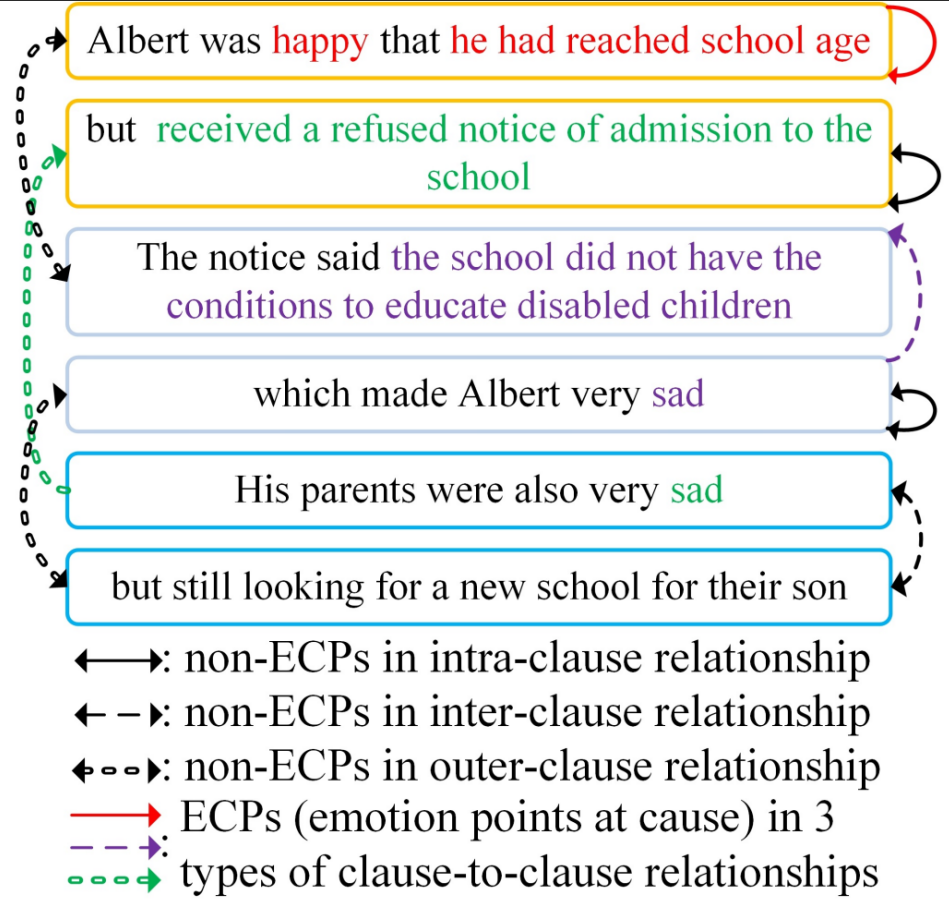
\includegraphics[width=0.55\linewidth]{figures/example.png}
% 	\caption{情感和原因通常相互关联,并且它们在一段文本中具有紧密的联系,研究此问题对计算机理解自然语言有着十分重要的作用。}
%     \label{fig:ecpe}
%     \vspace{7pt}
% \end{figure}

\begin{figure}[ht]
	\centering
    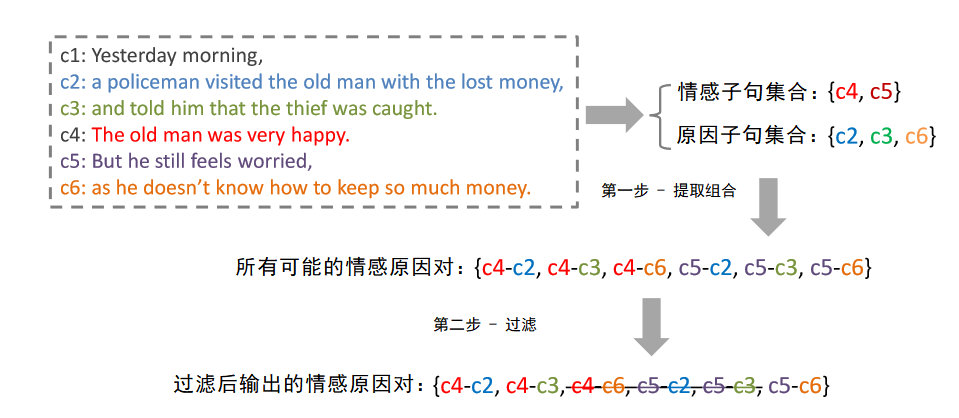
\includegraphics[width=0.95\linewidth]{figures/2step.png}
	\caption{情感和原因通常相互关联,并且它们在一段文本中具有紧密的联系,研究此问题对计算机理解自然语言有着十分重要的作用。本图展示了处理ECPE的传统的两步架构,分别抽取情感原因后再进行匹配,筛选出文本中潜在的情感原因对。}
    \label{fig:2step}
\end{figure}


情感和原因之间的子句级别关系由于其在实际应用中的有效性而受到了广泛关注。情绪原因对提取(Emotion-cause Pair Extraction, ECPE)任务是自然语言处理中的一个任务,其目的是从文本中自动抽取事件的因果关系。ECPE 任务通常包括三个子任务:事件抽取、句子分类和事件关系分类,旨在以子句对的形式从未注释的文本中同时提取潜在的情绪和对应的原因。


先前对ECPE的研究中,研究者 \upcite{DBLP:conf/acl/XiaD19} 为Inter-CE和Inter-EC设置了上界实验,以进一步探索这两个子任务的共享预测效果。在这些实验中,Inter-CE-Bound和Inter-EC-Bound分别使用原因抽取和情感抽取的标签来帮助另一个子任务。这两个变体都取得了更好的性能表现,特别是Inter-EC-Bound在原因提取任务上的改进远远超过Inter-CE-Bound在情感提取任务上的改进。作者认为这是因为原因提取任务比情感提取任务更加困难,并且有更多的改进空间。说明情感提取任务较容易,低优先级。
另一项研究表明,情感的错误传递是影响性能的关键。传统算法算法提取情感原因通常包含两步,如图\ref{fig:2step}所示。在第一步中,分别抽取情感和原因,并在第二步中对所有情感和原因进行匹配,删除不合适的对,剩下的对即为正确的情感-原因对。然而,这种方法严重受错误传递问题所影响。如果第一步出现错误,例如在情感或原因抽取时出现了错误,那么这些错误将会影响第二步的匹配过程,进而影响最终的性能表现。


 
\BiSection{本文研究内容及结构安排}{Tables} 
\BiSubsection{本文研究内容}{}



本研究中主要探究了在多角色对话情感溯源任务上开展了ECPE的相关研究。
多角色对话情感溯源任务考虑到了对话中多个参与者的情感变化和相互作用,具有更高的难度和挑战性。此外还因此可以帮助研究者更好地理解对话数据集中的隐含信息,探索多角色对话情感变化的规律和特征。
同时,多角色对话情感溯源任务也有着广泛的应用价值。例如,可以应用于智能客服和情感智能交互系统中,以实现更加智能、自然和人性化的人机交互。
另外,多角色对话情感溯源任务还可以为心理学和社会学研究提供有益的数据支持,帮助研究者更好地理解人类情感变化和相互作用的机制\upcite{reccon}。本研究进行了广泛调研印证了该研究的可行性,对相关数据集进行了分析及处理。

为了解决\ref{sec:1.1}章节中提到的错误传递的问题,本研究设计了Dag-Rank模型,其是一种新颖而高效的信息提取方法,将情感原因对作为一个整体输出,以避免配对模块导致的误差导致性能下降。我们希望它可以将情感和原因的语义信息结合在一起,并考虑它们之间的交互作用。这样,模型可以更好地理解文本的含义,并在不同的语境下推断出正确的情感-原因对。

本研究所提出的方法针对对话数据集的特点设计了新颖的图神经网络,重点加强了从不同发言者的话语关系中提取信息特征的能力。
本研究从排名的角度来处理情感-原因对的提取,即在给定文档中对子句对候选项进行排名,并在一种强调子句间建模的一步法来执行端到端的提取。
我们将每个话语视为一个图节点,并利用RoBERTa-Base 预训练语言模型 \cite{liu2019roberta}  提取特征。为确保模型准确性,在训练邻域对话图模型时则冻结模型参数。我们采用类似于注意力聚合的方法对节点间信息进行整合,以更新节点信息。通过堆叠图模块,我们利用GRU实现各节点信息与在上一层的隐藏状态进行交互,增强了模型表征能力。我们通过跨层信息传递使模型能够接受遥远信息的影响,从而促进通过捕获两个子句之间的潜在关系来进行对提取。
然后,它学习子句对表示并对这些对进行排名以提取情感-原因对。本研究使用了一个基于核函数的相对位置嵌入方案来模拟相对位置之间的相互影响,并增强子句对表示以进行有效的排名。我们将这两个组件集成到一个统一的神经网络中,该网络被端到端地优化。与先前的两步解决方案不同,本研究所提出的Dag-Rank方法可以直接从文档中提取情感-原因对。

本文在现有数据集上进行了充分的的实验,与先进方法进行了对比;本研究包含了广泛的消融实验,证明了我们的设计具有良好的创新性和合理性,表现出了很好的性能。
实验证明,本研究设计的方法针对对话数据集具有很好的适用性。Dag-Rank模型能够充分提取对话文本中的感情因素,为错误传递问题提供了一个很好的解决方案。我们的模型能够更好地考虑到每个话语的上下文信息,从而更准确地理解对话文本的语义信息。实验结果表明,我们的邻域对话图模型在多个对话数据集上都取得了显著的提升效果。我们的研究成果为ECPE任务的实现提供了一种新的高效方法,并在自然语言处理领域具有重要的应用前景。


\BiSubsection{本文结构安排}{}
本文共分为五个章节,具体结构安排如下:

第一章为绪论,主要介绍了本文的研究背景及意义,以及本文的研究内容和结构安排。

第二章为相关工作,主要介绍了自然语言处理、文本情感溯源和图神经网络等方面的相关工作。

第三章为我们基于图表示学习与排序的文本情感溯源方法,包含对文本情感溯源问题的定义和描述。主要介绍了该方法的具体实现过程,包括文本编码、有向图模型和排序方法等。

第四章为实验测试与分析,主要对本文提出的文本情感溯源方法进行了实验验证和分析。

第五章为结论与展望,对本文的研究工作进行了总结,并对未来的研究方向进行了展望。


%-----------------------------------------------------------------------------------------

\BiChapter{相关工作}{}
\BiSection{自然语言处理}{Subequations}

深度学习方法使用多个处理层来学习数据的层次表示,并在许多领域产生了最先进的结果。近年来,在自然语言处理(NLP)的背景下,各种模型设计和方法得到了蓬勃发展。

% \textit{\textbf{传统机器学习}}:
早期,传统方法如支持向量机(SVM)\cite{zhang2011comparative}和逻辑回归(Logistic Regression)\cite{genkin2007large}利用稀疏表示,例如词袋(BoW)和TF-IDF。然而,最近的研究专注于密集表示,以缓解稀疏表示的限制\upcite{lilleberg2015support, yin2015document, ren2016topic}。这些密集表示也可用作输入到复杂方法(例如Deep Averaging Networks(DAN)\cite{iyyer2015deep}和Paragraph Vector(Doc2Vec)\cite{le2014distributed})的输入,以实现新的最先进结果。

% \textit{\textbf{序列模型}}:
RNN和CNN已被用于从输入文本中捕获连续单词的局部语义和句法信息。升级的模型,例如LSTM \cite{graves2012long}和GRU \cite{cho2014learning},已被提出来解决由原始 RNN引起的梯度消失或爆炸问题。基于CNN的结构已用于通过使用一个或多个卷积和池化层来捕获N-gram特征,例如Dynamic CNN \cite{kalchbrenner2014convolutional}和TextCNN \cite{kim2014convolutional}。然而,这些模型只能捕获连续单词的局部依赖性。为了捕获更长期或非欧几里德关系,提出了改进的RNN结构,例如Tree-LSTM \cite{tai2015improved}和MT-LSTM \cite{liu2015multi},以及全局语义信息,例如TopicRNN \cite{dieng2016topicrnn}。此外,提出了增强了CNN的图形\cite{peng2018large}和树形结构\cite{mou2015natural},以学习更多全局和长期依赖关系。

% \textit{\textbf{注意力和Transformer}}:
注意力机制\cite{bahdanau2014neural}已被广泛采用来捕获长距离依赖关系,例如分层注意网络\cite{abreu2019hierarchical}和基于注意力的混合模型\cite{yang2016hierarchical}。基于自我注意力的 Transformer 模型通过在某些任务上进行预训练以生成强大的上下文单词表示,已在许多文本分类基准测试中实现了最先进的性能,如图\ref{fig:bert}。然而,这些模型仅关注学习输入文本体之间的关系,忽略全局和语料库级别的信息。研究人员已经提出了将注意力机制和图神经网络(GNNs)的优点相结合,以学习输入文本体之间的关系和全局和语料库级别的信息,例如 VGCN-BERT \cite{VGCNBERT2020}和BERTGCN \cite{BERTGCN2021}。


\begin{figure}[ht]
	\centering
    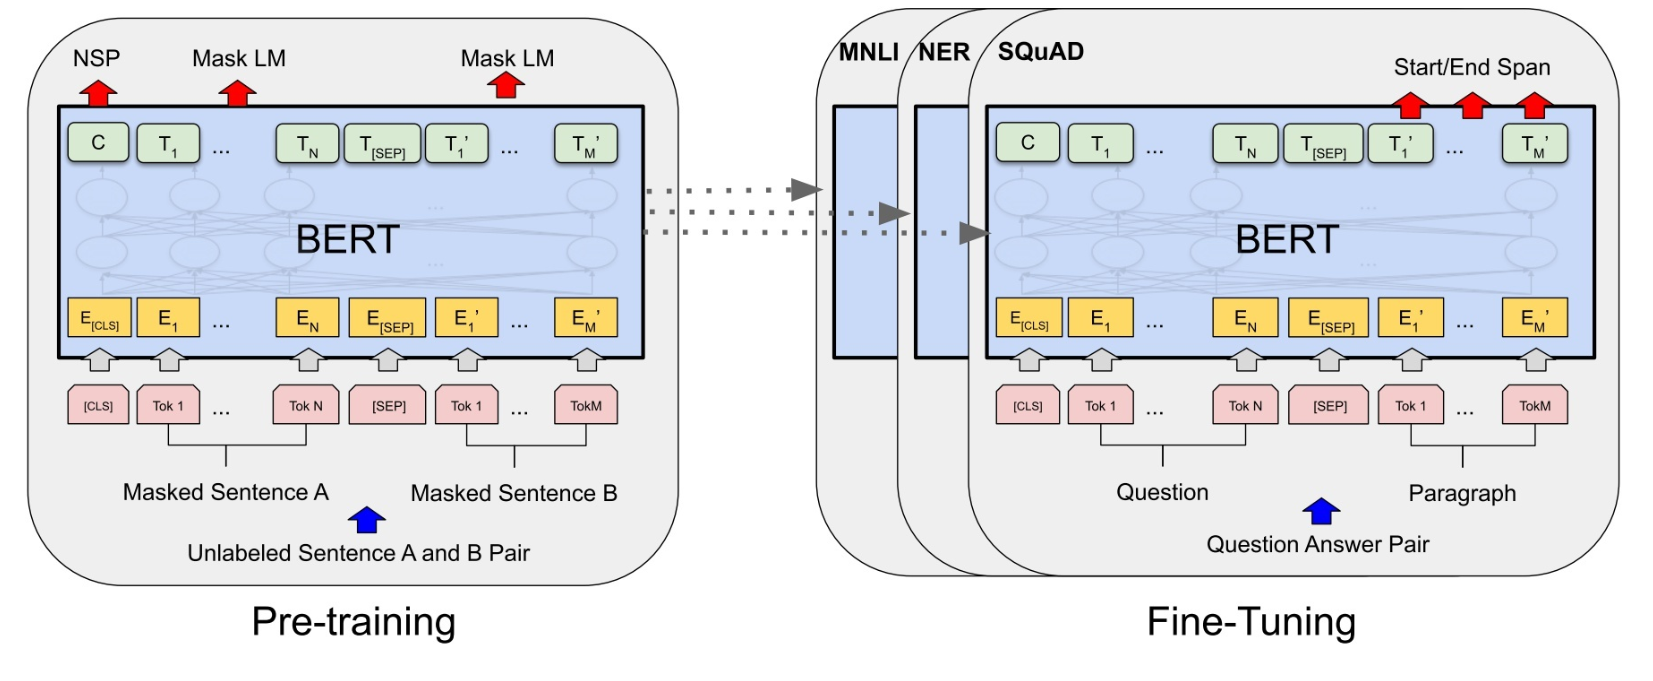
\includegraphics[width=0.95\linewidth]{figures/bert.png}
	\caption{BERT是一种自然语言处理预训练模型,它使用了Transformer结构进行编码,被广泛应用于自然语言推理、对话生成、问答系统等领域,并在多项开放数据集上取得了突出的表现。}
    \label{fig:bert}
\end{figure}



\BiSection{文本情感溯源}{Subequations}

在文章\cite{lee-etal-2010-text}中首次定义了情绪原因提取任务(Emotion Cause Extraction ECE),即从文本中提取给定情绪的词级原因。早期的ECE工作主要依赖于语言规则\upcite{lee-etal-2010-text,DBLP:conf/coling/ChenLLH10,DBLP:conf/nlpcc/GuiYXLLZ14}或传统的机器学习算法\cite{DBLP:conf/emnlp/GuiWXLZ16}。随着深度神经网络的发展,ECE任务的最近工作逐渐采用深度学习模型。
% 如共注意力\upcite{DBLP:conf/emnlp/LiSFWZ18}、自注意力\upcite{DBLP:conf/ijcai/XiaZD19}、多任务学习\upcite{DBLP:conf/emnlp/ChenHCL18}、图神经网络\upcite{DBLP:journals/kbs/HuLZ21}和外部知识的结合\upcite{DBLP:conf/acl/Yan0PH20}来解决这个任务。
具体来说,研究\cite{DBLP:conf/emnlp/ChenHCL18}将情绪分类和原因检测统一起来,充分利用情绪分类和原因检测之间的交互。研究\cite{DBLP:conf/emnlp/LiSFWZ18}考虑到情绪上下文的认知,构建了共注意力网络,将情绪信息融入到子句表示中。研究\cite{DBLP:conf/ijcai/XiaZD19}采用了Transformer\cite{DBLP:conf/nips/VaswaniSPUJGKP17}作为子句编码器,编码文档中子句之间的相互指示,以便基于这种全局信息提取情绪原因子句。

虽然ECE任务已经取得了重大进步,但它还存在两个缺点:1)在ECE任务中,必须在提取原因子句之前注释情绪;2)忽略了情绪和其对应的原因子句之间相互指示的事实。第一个问题严重限制了它在现实世界应用场景中的应用,第二个问题缺乏利用情绪和原因之间相互指示的优势。
为了解决这些缺点,基于ECE任务,最近发展出了情绪原因对提取(Emotion-cause Pair Extraction, ECPE)\cite{DBLP:conf/acl/XiaD19},如图\ref{fig:ecpe}。ECPE任务旨在以子句对的形式从未注释的文本中同时提取潜在的情绪和对应的原因。



\begin{figure}[ht]
	\centering
    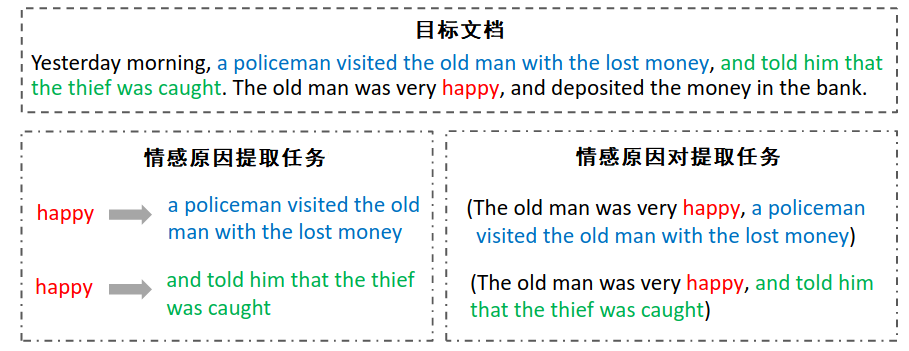
\includegraphics[width=0.95\linewidth]{figures/newtask.png}
	\caption{情绪原因对提取提取任务,旨在从文档中提取潜在的情绪和相应的原因对。}
    \label{fig:ecpe}
\end{figure}


对于ECPE任务,研究\cite{DBLP:conf/acl/XiaD19}提出了一个两步架构,第一步是构建情绪提取和原因提取之间的交互网络,以同时提取情绪和原因。第二步是通过分类由情绪和原因构建的对来过滤负对。这种两步方法是一个管道系统,可能会导致错误从第一步进一步传播到第二步。为了解决这个问题,研究\cite{DBLP:conf/acl/WeiZM20}采用了一个统一的架构,通过建模子句间的依赖关系,对对表示进行编码,并从排名的角度确定情绪-原因对。有研究\cite{DBLP:conf/acl/DingXY20}提出了2D-Transformer,将表示、交互和预测集成到一个联合框架中,以解决ECPE问题。有研究\cite{DBLP:conf/acl/FanYDGYX20}将ECPE视为一个类似解析的有向图构建过程,并基于一系列的行为生成了带有标记边的有向图。一些工作\cite{DBLP:conf/emnlp/YuanFBX20,DBLP:conf/coling/ChenLW20}使用序列标签方法来标记情绪-原因对。研究\cite{DBLP:journals/taslp/ChengJYLG21}从序列标注的角度解决了情绪-原因对提取任务,设计了一个内容标记来识别情绪/原因和一个配对标记来配对子句,这利用了目标子句、全局上下文和先前解码标签的信息,形成子句表示。研究\cite{DBLP:journals/taslp/FanYGZX21}提出了一个多任务序列标注框架,并使用两个辅助任务的预测分布作为归纳偏见来细化标签分布。某些研究者\cite{DBLP:conf/emnlp/ChenLW20}提出了一个新的任务,确定在不同的上下文中,情绪和原因子句是否有有效的因果关系,并基于现有的基准数据集通过手动注释和负采样构建了一个相应的数据集。


\BiSection{图神经网络}{Subequations}

图神经网络(Graph Neural Network, GNN)是一种可以处理图结构数据的深度学习模型,
它通过在节点之间传递和聚合信息来学习节点的表示。它的核心思想是将节点的特征信息与其邻居节点的信息进行交互和更新,从而获取节点的上下文信息。
GNN近年来在自然语言处理领域得到了广泛应用。它可以用于词语关系建模、句子关系建模\upcite{li2022survey}、文档分类\upcite{yin2015document}、命名实体识别\upcite{sui2022trigger}等任务。通过结合图结构的上下文信息,GNN能够捕捉到语义、句法和语境之间的关系,从而提升了文本处理任务的性能\upcite{DADGNN2021}。

% TODO:可以添加 GNN 基本方法
\subsection{图神经网络基础}
我们将图表示为 $G = (V, E)$,其中 $V$ 和 $E$ 分别表示 $G$ 的节点(顶点)和边的集合。节点集中的单个节点表示为 $v_i\in V$,边 $e_{ij}=(v_i, v_j)\in E$ 表示节点 $v_i$ 和 $v_j$ 之间的边。图 $G$ 的邻接矩阵表示为 $A$,其中 $A\in \mathbb{R}^{n\times n}$,$n$ 是图 $G$ 中节点的数量。如果 $e_{ij}\in E$,则 $A_{ij}=1$,否则 $A_{ij}=0$。此外,本研究使用 $\textbf{\textit{X}}$ 和 $\textbf{\textit{E}}$ 表示图 $G$ 中的节点和边的表示,其中 $\textbf{\textit{X}}\in \mathbb{R}^{n\times m}$,$\textbf{\textit{E}}\in \mathbb{R}^{n\times c}$。$\textbf{\textit{x}}_i\in \mathbb{R}^m$ 表示节点 $v_i$ 的 $m$ 维向量,$\textbf{\textit{e}}_{ij}\in \mathbb{R}^c$ 表示边 $e_{ij}$ 的 $c$ 维向量(最近的研究大多将 $c=1$ 作为加权标量的表示方式)。$\textbf{\textit{A}}$ 表示带权边特征的邻接矩阵。


为了解决传统基于图的算法的限制并更好地表示实际应用中的非欧几里得关系,研究\cite{GNN} 提出了图神经网络(Graph Neural Networks,GNNs)。GNNs 具有统一的基于图的框架,同时模拟图结构、节点和边的表示。本节将提供 GNN 的一般数学定义。GNN 的一般前向过程可以总结如下:
\begin{equation}
  \textbf{\textit{H}}^{(l)} =  \mathcal{F}(\textbf{\textit{A}},\textbf{\textit{H}}^{(l-1)})
\end{equation}
\vspace{1pt}
其中 $\textbf{\textit{A}}\in \mathbb{R}^{n\times n}$ 表示加权邻接矩阵,$\textbf{\textit{H}}^{(l)}\in \mathbb{R}^{n\times d}$ 是通过将 $l-1$ 层节点特征 $\textbf{\textit{H}}^{(l-1)}\in \mathbb{R}^{n\times k}$ ($k$ 是前一层节点表示的维度)输入预定义图滤波器 $\mathcal{F}$ 更新的第 $l$ 层 GNN 的节点表示。

最常用的图滤波方法定义如下:
\begin{equation}
  \textbf{\textit{H}}^{(l)} =  \phi(\tilde{\textbf{\textit{A}}}\textbf{\textit{H}}^{(l-1)}\textbf{\textit{W}})
\end{equation}
其中 $\tilde{\textbf{\textit{A}}}=\textbf{\textit{D}}^{-\frac{1}{2}}\textbf{\textit{AD}}^{-\frac{1}{2}}$ 是归一化的对称邻接矩阵。$\textbf{\textit{A}}\in \mathbb{R}^{n\times n}$ 是图 $G$ 的邻接矩阵,$\textbf{\textit{D}}$ 是 $\textbf{\textit{A}}$ 的度矩阵,其中 $D_{ii}=\sum_{j}A_{ij}$。$\textbf{\textit{W}}\in \mathbb{R}^{k\times d}$ 是权重矩阵,$\phi$ 是激活函数。如果我们基于上述滤波器设计两层 GNN,可以得到一个用于文本分类的基本图卷积网络(Graph Convolutional Network,GCN)\cite{GCN} 框架:
\begin{equation}
  \textbf{\textit{Y}} =  softmax(\tilde{\textbf{\textit{A}}}(ReLU(\tilde{\textbf{\textit{A}}}\textbf{\textit{H}}\textbf{\textit{W}}^{(0)}))\textbf{\textit{W}}^{(1)})
\end{equation}
\vspace{1pt}
其中 $\textbf{\textit{W}}^0$ 和 $\textbf{\textit{W}}^1$ 分别表示不同的 GCN 层的权重矩阵,$\textbf{\textit{H}}$ 是输入节点特征。使用 $ReLU$ 函数进行非线性化,使用 $softmax$ 生成预测类别 $\textbf{\textit{Y}}$。


\subsection{基于图的自然语言处理算法}
% 在广泛使用 GNN 表示不规则关系之前,传统的基于图的算法已经被应用于模拟文本分类中的非欧几里得结构,例如随机游走\upcite{szummer2001partially,zhou2005text},图匹配\upcite{schenker2004classification, silva2014bog},图聚类\upcite{matsuo2006graph},这些在\upcite{wu2021graph}中有很好的总结。这些传统基于图的算法存在三个常见的限制。首先,大多数算法主要关注捕获图层次结构的信息,而忽略节点和边特征的重要性。例如,基于随机游走的方法\upcite{zhou2005text,szummer2001partially}主要关注使用节点向量之间的距离或角度来计算转移概率,而忽略了节点向量所代表的信息。其次,由于传统基于图的算法仅适用于特定的任务,因此没有统一的学习框架来解决各种实际任务。例如,\upcite{kaur2018domain}提出了一种图聚类方法,需要基于领域知识的本体图。最后,传统的基于图的方法比较耗费时间,例如基于图编辑距离的图匹配方法具有指数时间复杂度\upcite{silva2014bog}。

基于 GNN 的自然语言处理模型通常包括两个步骤:对文本进行表示和对表示进行后处理。其中,对文本进行表示的方法通常是将文本转化为图结构数据,以便于利用 GNN 进行学习和推理。
GCN、GraphSAGE和GAT是常见的GNN模型。GCN和GraphSAGE均将实体和关系表示为知识图谱中的节点和边,并使用不同的聚合方法对节点进行更新,生成实体和关系的表示,最后利用分类器进行分类。GAT则使用注意力机制对节点进行聚合,生成实体和关系的表示,最后利用分类器进行分类。



\begin{figure}[ht]
    \vspace{6pt}
	\centering
    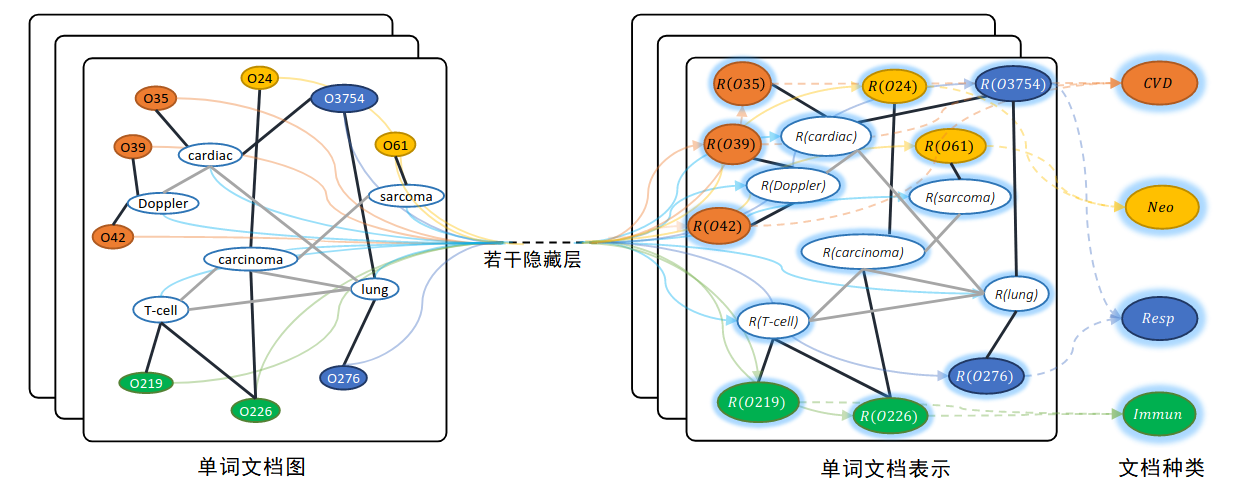
\includegraphics[width=\linewidth]{figures/textgcn.png}
	\caption{TextGCN是一种利用GCN来建模文本数据中文档之间关系的文本分类模型,它通过综合考虑文本内容和文档之间的相似度来生成准确的分类结果。}
    \label{fig:textgcn}
    \vspace{6pt}
\end{figure}


近期,许多基于GNN的自然语言处理方法被提出。TextGCN \cite{TEXTGCN2019}是一种基于GCN的文本分类模型,它将文本转化为一个无向图,每个节点表示一个文档,每个边表示文档之间的相似度。如图\ref{fig:textgcn}所示,对于每个文档,TextGCN使用CNN和GRU对文本序列进行编码,然后使用GCN对文档之间的关系进行建模,最后将GCN的输出作为分类器的输入生成最终分类结果。knn-GCN则利用K近邻图对文档之间的关系进行建模,并使用GCN和注意力机制对文档进行分类。
TextGTL\cite{TEXTGTL2021}则使用三种不同的文本图分别进行建模,其方法构建了三个不同的文档图:语义文本图、句法文本图和上下文文本图并分别使用不同的算法计算文档之间的关系,最后使用GCN对三个文本图进行学习和推理,生成最终的分类结果。
TG-Transformer\cite{TGTRANSFORMER2020}分别为文档节点和单词节点采用了两组权重。为了处理大型语料库图,使用PageRank算法\cite{page1999pagerank}从TextGCN图中采样子图。输入嵌入是三种类型嵌入的总和:预训练的GloVe嵌入、节点类型嵌入和Weisfeiler-Lehman结构编码\cite{niepert2016learning}。在传播过程中,应用了带图残差\cite{zhang2019gresnet}的自我注意力\cite{vaswani2017attention}。
BertGCN\cite{BERTGCN2021}\textbf{ }
为了结合BERT\cite{BERT}和TextGCN,BertGCN通过用每个时期的BERT [CLS]输出替换文档节点初始化,用零替换单词输入向量,以增强TextGCN。BertGCN通过插值TextGCN和BERT的输出来联合训练BERT和TextGCN:
\begin{equation}
\bm{Z} = \lambda\bm{Z}{GCN} + (1-\lambda)\bm{Z}{BERT}
\end{equation}
\vspace{1pt}
其中,$\lambda$是权衡因子。为了在训练过程中优化内存,使用了一个记忆库来跟踪文档输入,并将较小的学习率设置为BERT模块,以保持记忆库的一致性。BertGCN表明,在TextGCN的帮助下,BERT可以取得更好的性能。
研究\cite{HYPERGAT2020} 提出了 HyperGAT(超图注意力网络),为每个文档构建超图,以捕获单词之间的高级交互。包括两种类型的超边:连接句子中所有单词的顺序超边和使用 LDA 获取每个单词的主题后连接前 K 个单词的语义超边。像传统的超图传播一样,HyperGAT 遵循相同的两步更新步骤,但使用注意力机制来突出关键信息:节点级注意力用于学习超边表示,边级注意力用于更新节点表示。
% IGCN\upcite{IGCN2020} \textbf{ }
% 上下文依赖关系有助于理解文档。IGCN 使用依赖图构建图,以显示文档中每对单词的连通性。然后,使用 POS 嵌入和单词嵌入从 Bi-LSTM 学习的单词表示用于计算每对节点之间的相似性。注意力用于输出,以找到重要的相关语义特征。
% GTNT\upcite{GTNT2021}\textbf{ }的研究者们认为,TF-IDF 值较高的单词应连接更多的单词节点。因此,GTNT 使用排序后的 TF-IDF 值来确定每个节点的度,并应用 Havel-Hakimi 算法\upcite{hakami1962realizability}来确定单词节点之间的边。在模型学习过程中,应用了 GAT 的变种。尽管 GAT 的注意力得分对两个节点来说是相互的,但 GTNT 使用相关重要性来调整从一个节点到另一个节点的注意力得分。预训练的 Word2vec 作为每个节点的输入。

综上所述,图神经网络作为一种新兴的深度学习模型,在自然语言处理中得到了广泛的应用。不同的 GNN 模型适用于不同的任务,如文本分类\upcite{TEXTLEVELGNN2019,GNNXML2020,MLGNN2021}、实体关系抽取\upcite{sui2022trigger}、问题答案匹配\upcite{yasunaga2021qa}等。随着研究者们的不断探索,图神经网络在自然语言处理中的应用将会越来越广泛。



%=========================================================================================

